\section{Обзор IBM LSF} 

% The IBM Spectrum LSF ("LSF", short for load sharing facility) software is industry-leading enterprise-class software. LSF distributes work across existing heterogeneous IT resources to create a shared, scalable, and fault-tolerant infrastructure, that delivers faster, more reliable workload performance and reduces cost. LSF balances load and allocates resources, and provides access to those resources.
Программное обеспечение IBM Spectrum LSF («LSF», сокращенно от load sharing facility --- средства распределения нагрузки) является ведущим в отрасли программным обеспечением корпоративного класса. LSF распределяет работу по существующим разнородным компьютерным ресурсам для создания общей, масштабируемой и отказоустойчивой инфраструктуры, которая обеспечивает более быструю и надежную производительность рабочих нагрузок и снижает затраты. LSF балансирует нагрузку и распределяет ресурсы, а также обеспечивает доступ к этим ресурсам \cite{lsf_overview}. 

% LSF provides a resource management framework that takes your job requirements, finds the best resources to run the job, and monitors its progress. Jobs always run according to host load and site policies.
LSF предоставляет фреймворк управления ресурсами, которая учитывает необходимые ресурсы для задания, находит лучшие ресурсы для выполнения задания и отслеживает его выполнение. Задания всегда выполняются в соответствии с нагрузкой на хост и политикой планировщика.

\begin{figure}[h]
    \centering
    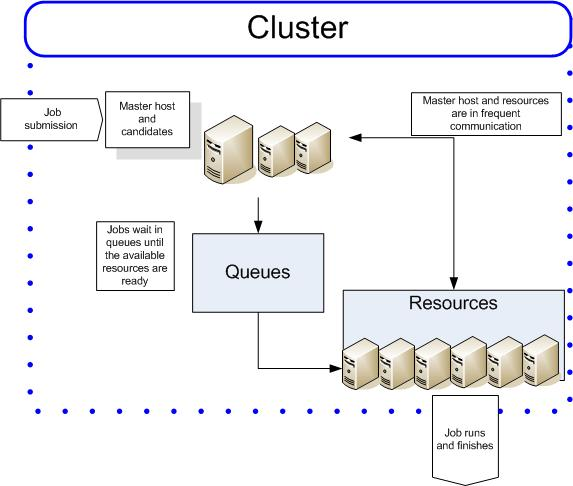
\includegraphics[width=\linewidth]{lsf_cluster_overview.jpg}
    \caption{Кластер LSF}
    \label{fig:LSF_cluster}
\end{figure}

\subsection{Кластер}

% A group of computers (hosts) running LSF that work together as a single unit, combining computing power, workload, and resources. A cluster provides a single-system image for a network of computing resources.
Группа компьютеров (хостов), на которых запущен LSF, которые работают вместе как единое целое, объединяя вычислительную мощность, рабочую нагрузку и ресурсы. Кластер предоставляет образ одной системы для сети вычислительных ресурсов (рис. \ref{fig:LSF_cluster}).

% Hosts can be grouped into a cluster in a number of ways. A cluster can contain:
Хосты можно объединить в кластер несколькими способами. Кластер может содержать:

\begin{itemize}
    % \item All the hosts in a single administrative group
    % \item All the hosts on a subnetwork
    \item Все хосты в единой административной группе;
    \item Все хосты в подсети.
\end{itemize}

\subsection{Задача}

% A unit of work that is running in the LSF system. A job is a command that is submitted to LSF for execution. LSF schedules, controls, and tracks the job according to configured policies.
Единица работы, выполняемая в системе LSF. Задача --- это команда, которая отправляется LSF для выполнения. LSF планирует, контролирует и отслеживает задачу в соответствии с настроенными политиками.

% Jobs can be complex problems, simulation scenarios, extensive calculations, or anything that needs compute power.
Задачи могут представлять собой сложные задачи, сценарии моделирования, обширные вычисления или все, что требует вычислительной мощности.

\subsection{Слот задачи}

% A job slot is a bucket into which a single unit of work is assigned in the LSF system.
Слот задачи --- это гнездо, которому в системе LSF назначается отдельная единица работы.

% Hosts can be configured with multiple job slots and you can dispatch jobs from queues until all the job slots are filled. You can correlate job slots with the total number of CPUs in the cluster.
Хосты могут быть настроены с несколькими слотами, и вы можете отправлять задачи из очередей до тех пор, пока все слоты не будут заполнены. Вы можете соотнести слоты с общим количеством процессоров в кластере.

\subsection{Очередь}

% A cluster-wide container for jobs. All jobs wait in queues until they are scheduled and dispatched to hosts.
Контейнер для рабочих мест во всём кластере. Все задачи ожидают в очередях, пока они не будут запланированы и отправлены на хосты.

% Queues do not correspond to individual hosts; each queue can use all server hosts in the cluster, or a configured subset of the server hosts.
Очереди не соответствуют отдельным хостам; каждая очередь может использовать все хосты серверов в кластере или заданное подмножество хостов серверов.

% When you submit a job to a queue, you do not need to specify an execution host. LSF dispatches the job to the best available execution host in the cluster to run that job.
Когда вы отправляете задачу в очередь, вам не нужно указывать хост выполнения. LSF отправляет задачу на лучший доступный хост исполнения в кластере для выполнения этой задачи.

% Queues implement different job scheduling and control policies.
Очереди реализуют различные политики планирования задач и управления.

\subsection{Ресурсы}

% Resources are the objects in your cluster that are available to run work. For example, resources include but are not limited to hosts, CPU slots, and licenses.
Ресурсы --- это объекты в вашем кластере, которые доступны для выполнения работы. Например, ресурсы включают, помимо прочего, хосты, слоты процессоров и лицензии.

\lstset{emphstyle=\itshape}
\lstset{emph={cluster_name}}
\subsection{Хосты}

% A host is an individual computer in the cluster.
Хост --- это отдельный компьютер в кластере.

% Each host may have more than 1 processor. Multiprocessor hosts are used to run parallel jobs. A multiprocessor host with a single process queue is considered a single machine, while a box full of processors that each have their own process queue is treated as a group of separate machines.
У каждого хоста может быть более 1 процессора. Многопроцессорные хосты используются для выполнения параллельных задач. Многопроцессорный хост с единственной очередью считается отдельной машиной, в то время как коробка, полная процессоров, каждый из которых имеет свою собственную очередь процессов, рассматривается как группа отдельных машин \cite{hosts_about}.

% Hosts in your cluster perform different functions:
Хосты в вашем кластере выполняют разные функции:

\begin{itemize}
    % \item Management host --- LSF server host that acts as the overall coordinator for the cluster, doing all job scheduling and dispatch.
    % \item Server host --- A host that submits and runs jobs.
    % \item Client host --- A host that only submits jobs and tasks.
    % \item Execution host --- A host that runs jobs and tasks.
    % \item Submission host --- A host from which jobs and tasks are submitted.
    \item Хост управления --- хост север LSF, который действует как всеобщий координатор для кластера, выполняя планирование и отправку всех заданий из очередей в хосты исполнения;
    \item Хост сервер --- хост, который отправляет и запускает задачи;
    \item Хост клиент --- хост, который только отправляет задачи и задания;
    \item Хост исполнения --- хост, на котором выполняются задачи и задания;
    \item Хост отправки --- хост, с которого отправляются задачи и задания.
\end{itemize}

Команды:

\begin{itemize}
    % \item \lstinline{lsload} — View load on hosts
    % \item \lstinline{lshosts} — View configuration information about hosts in the cluster including number of CPUS, model, type, and whether the host is a client or server
    % \item \lstinline{bhosts} — View batch server hosts in the cluster
    \item \lstinline{lsload} --- просмотр нагрузки на хосты;
    \item \lstinline{lshosts} --- просмотр информации о конфигурации хостов в кластере, включая количество процессоров, модель, тип и то, является ли хост клиентом или сервером;
    \item \lstinline{bhosts} --- просмотр хостов пакетного сервера в кластере.
\end{itemize}

% Tip: The names of your hosts should be unique. They should not be the same as the cluster name or any queue defined for the cluster.
Совет: имена ваших хостов должны быть уникальными. Они не должны совпадать с именем кластера или какой-либо очередью, заданной для кластера.

\subsection{Хост отправки}

% The host where jobs are submitted to the cluster.
Хост, на котором задания отправляются в кластер.

% Jobs are submitted using the \lstinline{bsub} command or from an application that uses the LSF API.
Задания отправляются с помощью команды \lstinline{bsub} или из приложения, которое использует API LSF.

% Client hosts and server hosts can act as submission hosts.
Хосты клиенты и хосты серверы могут действовать как хосты отправки.

Команды:

\begin{itemize}
    % \item \lstinline{bsub} — Submit a job
    % \item \lstinline{bjobs} — View jobs that are submitted
    \item \lstinline{bsub} --- отправить задачу;
    \item \lstinline{bjobs} --- просмотр отправленных задач.
\end{itemize}

\subsection{Хост исполнения}

% The host where a job runs. Can be the same as the submission host. All execution hosts are server hosts.
Хост, на котором выполняется задание. Может быть тем же, что и хост отправки. Все хосты исполнения являются хостами серверами.

Команды:

\begin{itemize}
    % \item \lstinline{bjobs} — View where a job runs
    \item \lstinline{bjobs} --- просмотр, где запущена задача.
\end{itemize}

\subsection{Хост сервер}

% Hosts that are capable of submitting and executing jobs. A server host runs \lstinline{sbatchd} to execute server requests and apply local policies.
Хосты, которые могут отправлять и исполнять задания. Хост сервер запускает \lstinline{sbatchd} для исполнения запросов к серверу и применения локальных политик.

Команды:

\begin{itemize}
    % \item \lstinline{lshosts} — View hosts that are servers (server=Yes)
    \item \lstinline{lshosts} --- просмотр хостов серверов (\lstinline{server=Yes}).
\end{itemize}

Настройка:

\begin{itemize}
    % \item Server hosts are defined in the \lstinline{lsf.cluster.cluster_name} file by setting the value of server to 1
    \item Хосты сервера определяются в файле \lstinline{lsf.cluster.cluster_name} путем указания значения 1 для \lstinline{server}.
\end{itemize}


\subsection{Хост клиент}

% Hosts that are only capable of submitting jobs to the cluster. Client hosts run LSF commands and act only as submission hosts. Client hosts do not execute jobs or run LSF daemons.
Хосты, которые могут только отправлять задания в кластер. Хосты клиенты запускают команды LSF и действуют только как хосты отправки. Хосты клиенты не выполняют задания и не запускают демонов LSF (программы, работающие в фоновом режиме).

Команды:

\begin{itemize}
    % \item lshosts — View hosts that are clients (server=No)
    \item \lstinline{lshosts} --- просмотр хостов клиентов (\lstinline{server=No}).
\end{itemize}

Настройка:

\begin{itemize}
    % \item Client hosts are defined in the \lstinline{lsf.cluster.cluster_name} file by setting the value of server to 0
    \item Хосты клиенты определяются в файле \lstinline{lsf.cluster.cluster_name} путем указания значения 0 для \lstinline{server}.
\end{itemize}

\subsection{Хост управления}

% Where the master LIM and mbatchd run. An LSF server host that acts as the overall coordinator for that cluster. Each cluster has one master host to do all job scheduling and dispatch. If the master host goes down, another LSF server in the cluster becomes the master host.
Главный хост, где запускаются главный LIM и \lstinline{mbatchd}. Хост сервер LSF, который действует как всеобщий координатор для этого кластера. В каждом кластере есть один главный хост, который выполняет планирование и отправку всех заданий из очередей в хосты исполнения. Если главный хост выходит из строя, другой сервер LSF в кластере становится главным хостом.

% All LSF daemons run on the master host. The LIM on the master host is the master LIM.
Все демоны LSF работают на главном хосте. LIM на главном хосте является главным LIM.

Команды:

\begin{itemize}
    % \item \lstinline{lsid} — View the master host name
    \item \lstinline{lsid} --- просмотр имени главного хоста.
\end{itemize}

Конфигурация:

\begin{itemize}
    % \item The master host is the first host listed in the \lstinline{lsf.cluster.cluster_name} file or is defined along with other candidate master hosts by \lstinline{LSF_MASTER_LIST} in \lstinline{lsf.conf}.
    \item Главный хост --- это первый хост, указанный в файле \lstinline{lsf.cluster.cluster_name} или определенный вместе с другими хостами кандидатами в главные хосты в \lstinline{LSF_MASTER_LIST} в \lstinline{lsf.conf}.
\end{itemize}
\lstset{emph={}}

\clearpage